\documentclass{beamer}
%
% Choose how your presentation looks.
%
% For more themes, color themes and font themes, see:
% http://deic.uab.es/~iblanes/beamer_gallery/index_by_theme.html
%
\mode<presentation>
{
  \usetheme{default}      % or try Darmstadt, Madrid, Warsaw, ...
  \usecolortheme{default} % or try albatross, beaver, crane, ...
  \usefonttheme{default}  % or try serif, structurebold, ...
  \setbeamertemplate{navigation symbols}{}
  \setbeamertemplate{caption}[numbered]
  \setbeamertemplate{footline}[frame number]
  \setbeamertemplate{itemize items}[circle]
%   \setbeamertemplate{theorems}[numbered]
  \setbeamercolor*{structure}{bg=white,fg=blue}
  \setbeamerfont{block title}{size=\normalsize}
  \setbeamercolor{bibliography entry author}{fg=black}
  \setbeamercolor{bibliography entry title}{fg=black}
  \setbeamercolor{bibliography entry note}{fg=black}
}

% \newtheorem{proposition}[theorem]{Proposition}
% \theoremstyle{definition}
% \newtheorem{algorithm}[theorem]{Algorithm}
% \newtheorem{idea}[theorem]{Idea}

\usepackage[english]{babel}
\usepackage[utf8]{inputenc}
\usepackage[T1]{fontenc}
\usepackage{nicefrac}
% \usepackage{tabularx}
% \usepackage{makecell}
% \usepackage{amsmath,amsfonts,amsthm,amssymb,mathrsfs,bbm,mathtools}
% \usepackage{enumitem}
\usepackage{tikz}
% \usetikzlibrary{patterns}
% \usetikzlibrary{intersections}
% \usepackage{pgfplots}
% \usepgfplotslibrary{fillbetween}
% \usepgfplotslibrary{dateplot}
% \usepackage{pgfplotstable}

% \usepackage{booktabs}
% \usepackage[final]{microtype}
% \usepackage{caption}
% \usepackage{amsmath}
% \usepackage{mathtools}
% \usepackage{amsthm,thmtools}
% % \usepackage[nottoc]{tocbibind}
% % \usepackage[ruled]{algorithm2e}
% \usepackage{enumerate}
% \usepackage[italic]{esdiff}
% \usepackage{subcaption}
% \usepackage{ltablex}
% \usepackage{multirow}

%--------Pseudocode--------
\usepackage{xcolor,amsmath}
\usepackage{algorithm2e}
\DontPrintSemicolon
% \SetAlgoSkip{bigskip}

% % Define pseudocode formatting
% \renewcommand{\KwSty}[1]{\textnormal{\textcolor{blue!90!black}{\ttfamily\bfseries #1}}\unskip}
% \renewcommand{\ArgSty}[1]{\textnormal{\ttfamily #1}\unskip}
% \SetKwComment{Comment}{\color{green!50!black}// }{}
% \renewcommand{\CommentSty}[1]{\textnormal{\ttfamily\color{green!50!black}#1}\unskip}
% \newcommand{\assign}{\leftarrow}
% % \newcommand{\var}{\texttt}
% \newcommand{\FuncCall}[2]{\texttt{\bfseries #1(#2)}}
% \SetKwProg{Function}{function}{}{}
% \renewcommand{\ProgSty}[1]{\texttt{\bfseries #1}}

% % Settings for pgfplots
% \pgfplotsset{compat=newest}

% \renewcommand\tabularxcolumn[1]{m{#1}}
% \newcolumntype{R}{>{\raggedleft\arraybackslash}X}=

% \def\code#1{\texttt{\frenchspacing#1}}
\def\padding{\vspace{0.5cm}}
\def\spadding{\vspace{0.25cm}}
\def\b{\textcolor{blue}}
\def\r{\textcolor{red}}
\def\g#1{{\usebeamercolor[fg]{block title example}{#1}}}
\definecolor{softgreen}{RGB}{124,216,23}

% fix for \pause in align
\makeatletter
\let\save@measuring@true\measuring@true
\def\measuring@true{%
  \save@measuring@true
  \def\beamer@sortzero##1{\beamer@ifnextcharospec{\beamer@sortzeroread{##1}}{}}%
  \def\beamer@sortzeroread##1<##2>{}%
  \def\beamer@finalnospec{}%
}
\makeatother

% \DeclarePairedDelimiter{\norm}{\lVert}{\rVert}
\NewDocumentCommand{\follows}{}{\ensuremath{\rightsquigarrow}\hspace{0.5em}}
\newcommand*{\defeq}{\overset{.}{=}}
\newcommand*{\eqdef}{\overset{.}{=}}
\RenewDocumentCommand{\Pr}{om}{Pr\IfValueT{#1}{_{#1}}{}[#2]}
\NewDocumentCommand{\E}{om}{\mathbb{E}\IfValueT{#1}{_{#1}}{}#2}
\RenewDocumentCommand{\O}{m}{\mathcal{O}(#1)}
\NewDocumentCommand{\B}{}{\mathcal{B}}
\NewDocumentCommand{\G}{}{\mathcal{G}}
\RenewDocumentCommand{\L}{}{\r{\ensuremath{\mathcal{L}_\tau}}}
\NewDocumentCommand{\U}{}{\b{\ensuremath{\mathcal{U}_\tau}}}
\NewDocumentCommand{\pmax}{}{p_\mathrm{max}}
\NewDocumentCommand{\taumax}{}{\ensuremath{\tau_\mathrm{max}}}
\NewDocumentCommand{\var}{m}{\mathrm{var}(#1)}
\NewDocumentCommand{\maxsize}{m}{\mathrm{maxsize}(#1)}
\NewDocumentCommand{\poly}{m}{\mathrm{poly}(#1)}
\NewDocumentCommand{\law}{}{p}
\NewDocumentCommand{\w}{}{\ensuremath{w_\law}}
\NewDocumentCommand{\epsw}{}{\ensuremath{w_{\law^{1-\epsilon}}}}
\NewDocumentCommand{\compat}{mm}{#1[#2]}

\usepackage[sorting=ynt,style=alphabetic]{biblatex}
\addbibresource{sources.bib}

\renewcommand{\footnotesize}{\tiny}

\begin{document}

\title[Deterministic Algorithms for the Lovász Local Lemma]{Deterministic Algorithms \\ for the Lovász Local Lemma\footfullcite{harris2022deterministic}}
\author{Jonas Hübotter and Duri Janett \\ Advised by Yassir Akram}
\date{March 29, 2022}

\begin{frame}
  \titlepage
\end{frame}

% \begin{frame}{Outline}
%  \tableofcontents[subsubsectionstyle=hide,pausesections]
% \end{frame}
% \AtBeginSection[]
%   {
%      \begin{frame}[allowframebreaks]{Plan}
%      \tableofcontents[currentsection, sectionstyle=show/hide, hideothersubsections]
%      \end{frame}
%   }

\section{Introduction}
\subsection{Lovász Local Lemma and the MT Algorithm}
\begin{frame}{Setting}
Distribution $D$ over independent $\Sigma$-valued coordinates $X_1, \dots, X_n$.
``Bad-events'' $\B = \{B_1, \dots, B_m\}$, each a boolean function of some subset of coordinates $\var{B_i} \subseteq \{X_1,\dots,X_n\}$ with law $\law$.\pause

\begin{example}[3-SAT]
\begin{columns}
\begin{column}{.3\textwidth}
$\begin{aligned}
B_1 &\defeq f_1(X_1,X_3,X_5) \\
B_2 &\defeq f_2(X_2,X_3,X_6) \\
B_3 &\defeq f_3(X_1,X_5,X_6) \\
B_4 &\defeq f_4(X_2,X_4,X_7)
\end{aligned}$
\end{column}
\begin{column}{.3\textwidth}
\tikzset{every picture/.style={line width=0.75pt}} %set default line width to 0.75pt        

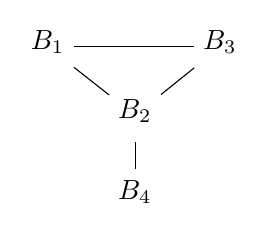
\begin{tikzpicture}[x=0.75pt,y=0.75pt,yscale=-1,xscale=1]
%uncomment if require: \path (0,534); %set diagram left start at 0, and has height of 534


% Text Node
\draw (20,22) node [anchor=north west][inner sep=0.75pt]    {$B_{1}$};
% Text Node
\draw (62,55) node [anchor=north west][inner sep=0.75pt]    {$B_{2}$};
% Text Node
\draw (103,22) node [anchor=north west][inner sep=0.75pt]    {$B_{3}$};
% Text Node
\draw (62,94) node [anchor=north west][inner sep=0.75pt]    {$B_{4}$};
% Connection
\draw    (100,31) -- (42,31) ;
% Connection
\draw    (59,54.18) -- (42,40.82) ;
% Connection
\draw    (84,53.94) -- (100,41.06) ;
% Connection
\draw    (71.5,77) -- (71.5,90) ;

\end{tikzpicture}
\end{column}
\end{columns}
\end{example}\pause

\begin{theorem}[(Symmetric) Lovász Local Lemma]
If for any $i$, $\law(B_i) \leq \pmax$ and $B_i$ affects at most $d$ bad-events, then $e \pmax d \leq 1$ implies $\Pr{\text{all $B_i$ avoided}} > 0$.
\end{theorem}\pause\spadding

For \g{$k$-SAT}, $\law \equiv 2^{-k}$ \follows satisfiable if any literal appears in $d \leq \nicefrac{2^k}{e}$ clauses!\pause\ How to find a satisfying assignment?
\end{frame}

\begin{frame}{Applications}
% TODO

\follows algorithmic versions of the Lovász Local Lemma yield automatic algorithms for these problems!
\end{frame}

\begin{frame}{Prior Work}
\begin{algorithm}[H]
    \TitleOfAlgo{MT-Algorithm}
    Draw $X$ from distribution $D$\;
    \While{some bad-event is true on $X$}{
        Select any true bad-event $B$\;
        For each $i \in \var{B}$, draw $X_i$ from its distribution in $D$\;
    }
\end{algorithm}\pause
\follows converges within $\O{m}$ iterations in expectation.\footfullcite{moser2010constructive}
\end{frame}

\subsection{Prior Work}
\begin{frame}{Prior Work}
What about deterministic algorithms?\pause\par
Polynomial-time algorithm if $e \pmax^{1-\epsilon} d \leq 1$ for any constant $\epsilon > 0$.\footfullcite{chandrasekaran2013deterministic}

% TODO
\end{frame}

\subsection{Overview of Results}
\begin{frame}{Contributions}
\begin{enumerate}
    \item \emph{Deterministic algorithm} with a simpler \& more general condition that is satisfied by \emph{most} variants of the LLL.\pause
    \item Faster \emph{parallel algorithm} with simpler conditions.\pause
    \item Algorithm that finds a configuration avoiding bad events such that the (weighted) probability of some auxiliary events is not much more than their expectation.
\end{enumerate}
\end{frame}

\section{Background}
\begin{frame}{Plan}
\tableofcontents[currentsection, sectionstyle=show/shaded, hideothersubsections]
\end{frame}

\subsection{Alternative Characterization of MT Algorithm}
\begin{frame}{Alternative Characterization of MT Algorithm}
Consider the \b{resampling table} $R$ drawn according to distribution $D$:\spadding

\begin{columns}
\begin{column}{.25\textwidth}



\tikzset{every picture/.style={line width=0.75pt}} %set default line width to 0.75pt        

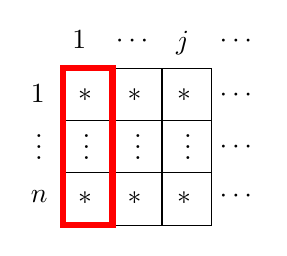
\begin{tikzpicture}[x=0.75pt,y=0.75pt,yscale=-1,xscale=1]
%uncomment if require: \path (0,534); %set diagram left start at 0, and has height of 534

%Shape: Rectangle [id:dp17271303952502315] 
% \draw   (52.81,325.2) -- (76.62,325.2) -- (76.62,350.41) -- (52.81,350.41) -- cycle ;
%Shape: Rectangle [id:dp4366577772656428] 
\draw   (76.81,350.41) -- (100.62,350.41) -- (100.62,375.62) -- (76.81,375.62) -- cycle ;
%Shape: Rectangle [id:dp13823281826780653] 
\draw   (76.81,325.2) -- (100.62,325.2) -- (100.62,350.41) -- (76.81,350.41) -- cycle ;
%Shape: Rectangle [id:dp25508926192152326] 
\draw   (100.62,325.2) -- (124.43,325.2) -- (124.43,350.41) -- (100.62,350.41) -- cycle ;
%Shape: Rectangle [id:dp7615695748694848] 
\draw   (124.43,325.2) -- (148.24,325.2) -- (148.24,350.41) -- (124.43,350.41) -- cycle ;
%Shape: Rectangle [id:dp7082057113045306] 
\draw   (100.62,350.41) -- (124.43,350.41) -- (124.43,375.62) -- (100.62,375.62) -- cycle ;
%Shape: Rectangle [id:dp5459336420864682] 
\draw   (124.43,350.41) -- (148.24,350.41) -- (148.24,375.62) -- (124.43,375.62) -- cycle ;
%Shape: Rectangle [id:dp8229762223203931] 
\draw   (76.81,375.62) -- (100.62,375.62) -- (100.62,400.83) -- (76.81,400.83) -- cycle ;
%Shape: Rectangle [id:dp7425833826219033] 
\draw   (100.62,375.62) -- (124.43,375.62) -- (124.43,400.83) -- (100.62,400.83) -- cycle ;
%Shape: Rectangle [id:dp11427372040336436] 
\draw   (124.43,375.62) -- (148.24,375.62) -- (148.24,400.83) -- (124.43,400.83) -- cycle ;
%Shape: Rectangle [id:dp835448558688529] 
\draw  [color={rgb, 255:red, 255; green, 0; blue, 0 }  ,draw opacity=1 ][line width=2.25]  (76.81,325.2) -- (100.62,325.2) -- (100.62,400.83) -- (76.81,400.83) -- cycle ;

% Text Node
\draw (82.82,334.01) node [anchor=north west][inner sep=0.75pt]    {$*$};
% Text Node
\draw (106.63,334.01) node [anchor=north west][inner sep=0.75pt]    {$*$};
% Text Node
\draw (130.44,334.01) node [anchor=north west][inner sep=0.75pt]    {$*$};
% Text Node
\draw (82.82,383.43) node [anchor=north west][inner sep=0.75pt]    {$*$};
% Text Node
\draw (106.63,383.43) node [anchor=north west][inner sep=0.75pt]    {$*$};
% Text Node
\draw (130.44,383.43) node [anchor=north west][inner sep=0.75pt]    {$*$};
% Text Node
\draw (62,348) node [anchor=north west][inner sep=0.75pt]    {$\vdots $};
% Text Node
\draw (60,332) node [anchor=north west][inner sep=0.75pt]    {$1$};
% Text Node
\draw (60,383) node [anchor=north west][inner sep=0.75pt]    {$n$};
% Text Node
\draw (85,348) node [anchor=north west][inner sep=0.75pt]    {$\vdots $};
% Text Node
\draw (109.81,348) node [anchor=north west][inner sep=0.75pt]    {$\vdots $};
% Text Node
\draw (133.81,348) node [anchor=north west][inner sep=0.75pt]    {$\vdots $};
% Text Node
\draw (80,306) node [anchor=north west][inner sep=0.75pt]    {$1$};
% Text Node
\draw (101,308) node [anchor=north west][inner sep=0.75pt]    {$\cdots $};
% Text Node
\draw (130,306) node [anchor=north west][inner sep=0.75pt]    {$j$};
% Text Node
\draw (151,308) node [anchor=north west][inner sep=0.75pt]    {$\cdots $};
% Text Node
\draw (151,334) node [anchor=north west][inner sep=0.75pt]    {$\cdots $};
% Text Node
\draw (151,359) node [anchor=north west][inner sep=0.75pt]    {$\cdots $};
% Text Node
\draw (151,383) node [anchor=north west][inner sep=0.75pt]    {$\cdots $};
% Text Node
% \draw (57.82,334.01) node [anchor=north west][inner sep=0.75pt]    {$*$};


\end{tikzpicture}
\vspace{0.15em}\pause
\end{column}\pause
\begin{column}{.1\textwidth}
\centering $\overset{\text{resampling $X_1$}}{\follows}$
\end{column}
\begin{column}{.3\textwidth}



\tikzset{every picture/.style={line width=0.75pt}} %set default line width to 0.75pt        

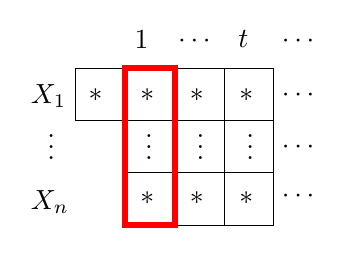
\begin{tikzpicture}[x=0.75pt,y=0.75pt,yscale=-1,xscale=1]
%uncomment if require: \path (0,534); %set diagram left start at 0, and has height of 534

%Shape: Rectangle [id:dp17271303952502315] 
\draw   (52.81,325.2) -- (76.62,325.2) -- (76.62,350.41) -- (52.81,350.41) -- cycle ;
%Shape: Rectangle [id:dp4366577772656428] 
\draw   (76.81,350.41) -- (100.62,350.41) -- (100.62,375.62) -- (76.81,375.62) -- cycle ;
%Shape: Rectangle [id:dp13823281826780653] 
\draw   (76.81,325.2) -- (100.62,325.2) -- (100.62,350.41) -- (76.81,350.41) -- cycle ;
%Shape: Rectangle [id:dp25508926192152326] 
\draw   (100.62,325.2) -- (124.43,325.2) -- (124.43,350.41) -- (100.62,350.41) -- cycle ;
%Shape: Rectangle [id:dp7615695748694848] 
\draw   (124.43,325.2) -- (148.24,325.2) -- (148.24,350.41) -- (124.43,350.41) -- cycle ;
%Shape: Rectangle [id:dp7082057113045306] 
\draw   (100.62,350.41) -- (124.43,350.41) -- (124.43,375.62) -- (100.62,375.62) -- cycle ;
%Shape: Rectangle [id:dp5459336420864682] 
\draw   (124.43,350.41) -- (148.24,350.41) -- (148.24,375.62) -- (124.43,375.62) -- cycle ;
%Shape: Rectangle [id:dp8229762223203931] 
\draw   (76.81,375.62) -- (100.62,375.62) -- (100.62,400.83) -- (76.81,400.83) -- cycle ;
%Shape: Rectangle [id:dp7425833826219033] 
\draw   (100.62,375.62) -- (124.43,375.62) -- (124.43,400.83) -- (100.62,400.83) -- cycle ;
%Shape: Rectangle [id:dp11427372040336436] 
\draw   (124.43,375.62) -- (148.24,375.62) -- (148.24,400.83) -- (124.43,400.83) -- cycle ;
%Shape: Rectangle [id:dp835448558688529] 
\draw  [color={rgb, 255:red, 255; green, 0; blue, 0 }  ,draw opacity=1 ][line width=2.25]  (76.81,325.2) -- (100.62,325.2) -- (100.62,400.83) -- (76.81,400.83) -- cycle ;

% Text Node
\draw (82.82,334.01) node [anchor=north west][inner sep=0.75pt]    {$*$};
% Text Node
\draw (106.63,334.01) node [anchor=north west][inner sep=0.75pt]    {$*$};
% Text Node
\draw (130.44,334.01) node [anchor=north west][inner sep=0.75pt]    {$*$};
% Text Node
\draw (82.82,383.43) node [anchor=north west][inner sep=0.75pt]    {$*$};
% Text Node
\draw (106.63,383.43) node [anchor=north west][inner sep=0.75pt]    {$*$};
% Text Node
\draw (130.44,383.43) node [anchor=north west][inner sep=0.75pt]    {$*$};
% Text Node
\draw (38,348) node [anchor=north west][inner sep=0.75pt]    {$\vdots $};
% Text Node
\draw (30,332) node [anchor=north west][inner sep=0.75pt]    {$X_1$};
% Text Node
\draw (30,383) node [anchor=north west][inner sep=0.75pt]    {$X_n$};
% Text Node
\draw (85,348) node [anchor=north west][inner sep=0.75pt]    {$\vdots $};
% Text Node
\draw (109.81,348) node [anchor=north west][inner sep=0.75pt]    {$\vdots $};
% Text Node
\draw (133.81,348) node [anchor=north west][inner sep=0.75pt]    {$\vdots $};
% Text Node
\draw (80,306) node [anchor=north west][inner sep=0.75pt]    {$1$};
% Text Node
\draw (101,308) node [anchor=north west][inner sep=0.75pt]    {$\cdots $};
% Text Node
\draw (130,306) node [anchor=north west][inner sep=0.75pt]    {$t$};
% Text Node
\draw (151,308) node [anchor=north west][inner sep=0.75pt]    {$\cdots $};
% Text Node
\draw (151,334) node [anchor=north west][inner sep=0.75pt]    {$\cdots $};
% Text Node
\draw (151,359) node [anchor=north west][inner sep=0.75pt]    {$\cdots $};
% Text Node
\draw (151,383) node [anchor=north west][inner sep=0.75pt]    {$\cdots $};
% Text Node
\draw (57.82,334.01) node [anchor=north west][inner sep=0.75pt]    {$*$};


\end{tikzpicture}

\end{column}
\begin{column}{.05\textwidth}
\end{column}
\end{columns}\pause

When resampling $B_i$, shift rows $\var{B_i}$ to left.\pause\padding

\follows MT algorithm deterministic with respect to resampling table!
\end{frame}

% \subsection{Outline}
% \begin{frame}{Outline}
%     Goal: Find a resampling table such that after poly. resamples all bad-events are avoided.\spadding
    
%     Idea: Choose $R$ such that the MT algorithm only performs resamples that the randomized variant is likely to perform.\pause\padding
    
%     \begin{enumerate}
%         \item Construct set of unlikely resamples of randomized MT algorithm.\pause
%         \item Use method of conditional expectations to find a resampling table $R$ such that all of these resamplings are avoided.\pause
%         \item Simulate MT algorithm using $R$.
%     \end{enumerate}
% \end{frame}

\subsection{Counting Resamples}
\begin{frame}{Counting Resamples}
Find an injective mapping from resamples to some ``countable'' structure.\pause

\begin{block}{Why may executions be long?}
Given a resampling table $R$, a \b{(partial) execution} of the MT algorithm is described by the sequence of resampled bad-events.\pause\spadding

\begin{columns}
\begin{column}{.15\textwidth}
\centering $B_1, B_2, B_3\onslide<4->{, \r{B_4}}$
\end{column}
\begin{column}{.05\textwidth}
\centering $\mapsto$
\end{column}\pause
\begin{column}{.2\textwidth}
\centering\only<-3>{


\tikzset{every picture/.style={line width=0.75pt}} %set default line width to 0.75pt        

\hspace{-1.3em}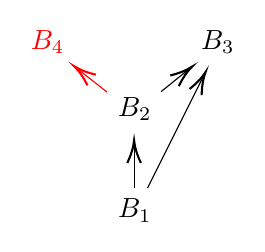
\begin{tikzpicture}[x=0.75pt,y=0.75pt,yscale=-1,xscale=1]
%uncomment if require: \path (0,534); %set diagram left start at 0, and has height of 534


% Text Node
\onslide<5->{\draw (241,27) node [anchor=north west][inner sep=0.75pt]  [color={rgb, 255:red, 255; green, 0; blue, 0 }  ,opacity=1 ]    {$B_{4}$};}
% Text Node
\draw (283,59) node [anchor=north west][inner sep=0.75pt]    {$B_{2}$};
% Text Node
\draw (323,27) node [anchor=north west][inner sep=0.75pt]    {$B_{3}$};
% Text Node
\draw (283,108) node [anchor=north west][inner sep=0.75pt]    {$B_{1}$};
% Connection
\onslide<5->{\draw [color={rgb, 255:red, 255; green, 0; blue, 0 }  ,draw opacity=1 ]    (279,57.79) -- (264.57,46.45) ;
\draw [shift={(263,45.21)}, rotate = 38.16] [color={rgb, 255:red, 255; green, 0; blue, 0 }  ][line width=0.75]    (10.93,-3.29) .. controls (6.95,-1.4) and (3.31,-0.3) .. (0,0) .. controls (3.31,0.3) and (6.95,1.4) .. (10.93,3.29)   ;}
% Connection
\draw    (305,57.54) -- (318.44,46.72) ;
\draw [shift={(320,45.46)}, rotate = 141.17] [color={rgb, 255:red, 0; green, 0; blue, 0 }  ][line width=0.75]    (10.93,-3.29) .. controls (6.95,-1.4) and (3.31,-0.3) .. (0,0) .. controls (3.31,0.3) and (6.95,1.4) .. (10.93,3.29)   ;
% Connection
\draw    (292,83) -- (292,104) ;
\draw [shift={(292,81)}, rotate = 90] [color={rgb, 255:red, 0; green, 0; blue, 0 }  ][line width=0.75]    (10.93,-3.29) .. controls (6.95,-1.4) and (3.31,-0.3) .. (0,0) .. controls (3.31,0.3) and (6.95,1.4) .. (10.93,3.29)   ;
% Connection
\draw    (298.5,104) -- (325.61,49.79) ;
\draw [shift={(326.5,48)}, rotate = 116.57] [color={rgb, 255:red, 0; green, 0; blue, 0 }  ][line width=0.75]    (10.93,-3.29) .. controls (6.95,-1.4) and (3.31,-0.3) .. (0,0) .. controls (3.31,0.3) and (6.95,1.4) .. (10.93,3.29)   ;

\end{tikzpicture}
}\only<4->{


\tikzset{every picture/.style={line width=0.75pt}} %set default line width to 0.75pt        

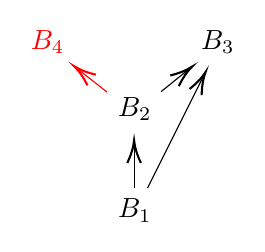
\begin{tikzpicture}[x=0.75pt,y=0.75pt,yscale=-1,xscale=1]
%uncomment if require: \path (0,534); %set diagram left start at 0, and has height of 534


% Text Node
\draw (241,27) node [anchor=north west][inner sep=0.75pt]  [color={rgb, 255:red, 255; green, 0; blue, 0 }  ,opacity=1 ]    {$B_{4}$};
% Text Node
\draw (283,59) node [anchor=north west][inner sep=0.75pt]    {$B_{2}$};
% Text Node
\draw (323,27) node [anchor=north west][inner sep=0.75pt]    {$B_{3}$};
% Text Node
\draw (283,108) node [anchor=north west][inner sep=0.75pt]    {$B_{1}$};
% Connection
\draw [color={rgb, 255:red, 255; green, 0; blue, 0 }  ,draw opacity=1 ]    (279,57.79) -- (264.57,46.45) ;
\draw [shift={(263,45.21)}, rotate = 38.16] [color={rgb, 255:red, 255; green, 0; blue, 0 }  ][line width=0.75]    (10.93,-3.29) .. controls (6.95,-1.4) and (3.31,-0.3) .. (0,0) .. controls (3.31,0.3) and (6.95,1.4) .. (10.93,3.29)   ;
% Connection
\draw    (305,57.54) -- (318.44,46.72) ;
\draw [shift={(320,45.46)}, rotate = 141.17] [color={rgb, 255:red, 0; green, 0; blue, 0 }  ][line width=0.75]    (10.93,-3.29) .. controls (6.95,-1.4) and (3.31,-0.3) .. (0,0) .. controls (3.31,0.3) and (6.95,1.4) .. (10.93,3.29)   ;
% Connection
\draw    (292,83) -- (292,104) ;
\draw [shift={(292,81)}, rotate = 90] [color={rgb, 255:red, 0; green, 0; blue, 0 }  ][line width=0.75]    (10.93,-3.29) .. controls (6.95,-1.4) and (3.31,-0.3) .. (0,0) .. controls (3.31,0.3) and (6.95,1.4) .. (10.93,3.29)   ;
% Connection
\draw    (298.5,104) -- (325.61,49.79) ;
\draw [shift={(326.5,48)}, rotate = 116.57] [color={rgb, 255:red, 0; green, 0; blue, 0 }  ][line width=0.75]    (10.93,-3.29) .. controls (6.95,-1.4) and (3.31,-0.3) .. (0,0) .. controls (3.31,0.3) and (6.95,1.4) .. (10.93,3.29)   ;

\end{tikzpicture}
}
\end{column}
\begin{column}{.3\textwidth}
\b{Witness DAG} $\hat{G}$

$B_i \longrightarrow B_j$ iff $i < j$\par and $B_i$ affects $B_j$
\end{column}
\end{columns}\pause\pause

\follows $\hat{G}$ is always a DAG!\pause\ But why use DAGs?
\end{block}
\end{frame}

\begin{frame}{Counting Resamples}
We can reconstruct the final configuration of the MT algorithm!\spadding

\begin{columns}[T]
\begin{column}{.4\textwidth}
\centering


\tikzset{every picture/.style={line width=0.75pt}} %set default line width to 0.75pt        

\begin{tikzpicture}[x=0.75pt,y=0.75pt,yscale=-1,xscale=1]
%uncomment if require: \path (0,534); %set diagram left start at 0, and has height of 534


% Text Node
\only<1-5,7-8>{\draw (241,27) node [anchor=north west][inner sep=0.75pt]    {$B_{4}$};}
\only<6,9->{\draw (241,27) node [anchor=north west][inner sep=0.75pt]  [color={rgb, 255:red, 255; green, 0; blue, 0 }  ,opacity=1 ]    {$B_{4}$};}
% Text Node
\only<1-3>{\draw (283,59) node [anchor=north west][inner sep=0.75pt]    {$B_{2}$};}
\only<4->{\draw (283,59) node [anchor=north west][inner sep=0.75pt]  [color={rgb, 255:red, 124; green, 216; blue, 23 }  ,opacity=1 ]    {$B_{2}$};}
% Text Node
\only<1-4,8-9>{\draw (323,27) node [anchor=north west][inner sep=0.75pt]    {$B_{3}$};}
\only<5-7,10->{\draw (323,27) node [anchor=north west][inner sep=0.75pt]  [color={rgb, 255:red, 250; green, 153; blue, 3 }  ,opacity=1 ]    {$B_{3}$};}
% Text Node
\only<1-2>{\draw (283,108) node [anchor=north west][inner sep=0.75pt]    {$B_{1}$};}
\only<3->{\draw (283,108) node [anchor=north west][inner sep=0.75pt]  [color={rgb, 255:red, 0; green, 0; blue, 255 }  ,opacity=1 ]    {$B_{1}$};}
% Connection
\draw    (279,57.79) -- (264.57,46.45) ;
\draw [shift={(263,45.21)}, rotate = 38.16] [color={rgb, 255:red, 0; green, 0; blue, 0 }  ][line width=0.75]    (10.93,-3.29) .. controls (6.95,-1.4) and (3.31,-0.3) .. (0,0) .. controls (3.31,0.3) and (6.95,1.4) .. (10.93,3.29)   ;
% Connection
\draw    (305,57.54) -- (318.44,46.72) ;
\draw [shift={(320,45.46)}, rotate = 141.17] [color={rgb, 255:red, 0; green, 0; blue, 0 }  ][line width=0.75]    (10.93,-3.29) .. controls (6.95,-1.4) and (3.31,-0.3) .. (0,0) .. controls (3.31,0.3) and (6.95,1.4) .. (10.93,3.29)   ;
% Connection
\draw    (292,83) -- (292,104) ;
\draw [shift={(292,81)}, rotate = 90] [color={rgb, 255:red, 0; green, 0; blue, 0 }  ][line width=0.75]    (10.93,-3.29) .. controls (6.95,-1.4) and (3.31,-0.3) .. (0,0) .. controls (3.31,0.3) and (6.95,1.4) .. (10.93,3.29)   ;
% Connection
\draw    (298.5,104) -- (325.61,49.79) ;
\draw [shift={(326.5,48)}, rotate = 116.57] [color={rgb, 255:red, 0; green, 0; blue, 0 }  ][line width=0.75]    (10.93,-3.29) .. controls (6.95,-1.4) and (3.31,-0.3) .. (0,0) .. controls (3.31,0.3) and (6.95,1.4) .. (10.93,3.29)   ;

\onslide<15->{\draw (228,73) node [anchor=north west][inner sep=0.75pt]  [color={rgb, 255:red, 255; green, 0; blue, 0 }  ,opacity=1 ]  {$\hat{G}(B_{4})$};

%Curve Lines [id:da02533473137358766] 
\draw [color={rgb, 255:red, 255; green, 0; blue, 0 }  ,draw opacity=1 ]   (260,24) .. controls (299,48) and (316,61) .. (309,110) ;
%Curve Lines [id:da2150259195395825] 
\draw [color={rgb, 255:red, 255; green, 0; blue, 0 }  ,draw opacity=1 ]   (244,48) .. controls (225,35) and (242,13) .. (260,24) ;
%Curve Lines [id:da46500745717824676] 
\draw [color={rgb, 255:red, 255; green, 0; blue, 0 }  ,draw opacity=1 ]   (244,48) .. controls (284,73) and (282,73) .. (279,107) ;
%Curve Lines [id:da9402495253404746] 
\draw [color={rgb, 255:red, 255; green, 0; blue, 0 }  ,draw opacity=1 ]   (309,110) .. controls (308,134) and (276,145) .. (279,107) ;}

\end{tikzpicture}
\spadding

{\small
\vspace{-2em}\begin{align*}
\var{B_1} = \{X_1,X_3,X_5\} \\
\var{B_2} = \{X_2,X_3,X_6\} \\
\var{B_3} = \{X_1,X_5,X_6\} \\
\var{B_4} = \{X_2,X_4,X_7\}
\end{align*}
}
\end{column}\pause
\begin{column}{.4\textwidth}
\centering


\tikzset{every picture/.style={line width=0.75pt}} %set default line width to 0.75pt        

\begin{tikzpicture}[x=0.75pt,y=0.75pt,yscale=-1,xscale=1,scale=0.75]
%uncomment if require: \path (0,534); %set diagram left start at 0, and has height of 534

%Shape: Rectangle [id:dp13823281826780653] 
\draw   (76.81,325.2) -- (100.62,325.2) -- (100.62,350.41) -- (76.81,350.41) -- cycle ;
%Shape: Rectangle [id:dp25508926192152326] 
\draw   (100.62,325.2) -- (124.43,325.2) -- (124.43,350.41) -- (100.62,350.41) -- cycle ;
%Shape: Rectangle [id:dp7615695748694848] 
\draw   (124.43,325.2) -- (148.24,325.2) -- (148.24,350.41) -- (124.43,350.41) -- cycle ;
%Shape: Rectangle [id:dp4366577772656428] 
\draw   (76.81,350.41) -- (100.62,350.41) -- (100.62,375.62) -- (76.81,375.62) -- cycle ;
%Shape: Rectangle [id:dp7082057113045306] 
\draw   (100.62,350.41) -- (124.43,350.41) -- (124.43,375.62) -- (100.62,375.62) -- cycle ;
%Shape: Rectangle [id:dp5459336420864682] 
\draw   (124.43,350.41) -- (148.24,350.41) -- (148.24,375.62) -- (124.43,375.62) -- cycle ;
%Shape: Rectangle [id:dp8229762223203931] 
\draw   (76.81,375.62) -- (100.62,375.62) -- (100.62,400.83) -- (76.81,400.83) -- cycle ;
%Shape: Rectangle [id:dp7425833826219033] 
\draw   (100.62,375.62) -- (124.43,375.62) -- (124.43,400.83) -- (100.62,400.83) -- cycle ;
%Shape: Rectangle [id:dp11427372040336436] 
\draw   (124.43,375.62) -- (148.24,375.62) -- (148.24,400.83) -- (124.43,400.83) -- cycle ;
%Shape: Rectangle [id:dp8229762223203931] 
\draw   (76.81,400.62) -- (100.62,400.62) -- (100.62,425.83) -- (76.81,425.83) -- cycle ;
%Shape: Rectangle [id:dp7425833826219033] 
\draw   (100.62,400.62) -- (124.43,400.62) -- (124.43,425.83) -- (100.62,425.83) -- cycle ;
%Shape: Rectangle [id:dp11427372040336436] 
\draw   (124.43,400.62) -- (148.24,400.62) -- (148.24,425.83) -- (124.43,425.83) -- cycle ;
%Shape: Rectangle [id:dp8229762223203931] 
\draw   (76.81,425.62) -- (100.62,425.62) -- (100.62,450.83) -- (76.81,450.83) -- cycle ;
%Shape: Rectangle [id:dp7425833826219033] 
\draw   (100.62,425.62) -- (124.43,425.62) -- (124.43,450.83) -- (100.62,450.83) -- cycle ;
%Shape: Rectangle [id:dp11427372040336436] 
\draw   (124.43,425.62) -- (148.24,425.62) -- (148.24,450.83) -- (124.43,450.83) -- cycle ;
%Shape: Rectangle [id:dp8229762223203931] 
\draw   (76.81,450.62) -- (100.62,450.62) -- (100.62,475.83) -- (76.81,475.83) -- cycle ;
%Shape: Rectangle [id:dp7425833826219033] 
\draw   (100.62,450.62) -- (124.43,450.62) -- (124.43,475.83) -- (100.62,475.83) -- cycle ;
%Shape: Rectangle [id:dp11427372040336436] 
\draw   (124.43,450.62) -- (148.24,450.62) -- (148.24,475.83) -- (124.43,475.83) -- cycle ;
%Shape: Rectangle [id:dp8229762223203931] 
\draw   (76.81,475.62) -- (100.62,475.62) -- (100.62,500.83) -- (76.81,500.83) -- cycle ;
%Shape: Rectangle [id:dp7425833826219033] 
\draw   (100.62,475.62) -- (124.43,475.62) -- (124.43,500.83) -- (100.62,500.83) -- cycle ;
%Shape: Rectangle [id:dp11427372040336436] 
\draw   (124.43,475.62) -- (148.24,475.62) -- (148.24,500.83) -- (124.43,500.83) -- cycle ;

% Text Node
\draw (81.82,332.01) node [anchor=north west][inner sep=0.75pt]    {$*$};
% Text Node
\draw (105.63,332.01) node [anchor=north west][inner sep=0.75pt]    {$*$};
% Text Node
\draw (129.44,332.01) node [anchor=north west][inner sep=0.75pt]    {$*$};
% Text Node
\draw (81.82,357.01) node [anchor=north west][inner sep=0.75pt]    {$*$};
% Text Node
\draw (105.63,357.01) node [anchor=north west][inner sep=0.75pt]    {$*$};
% Text Node
\draw (129.44,357.01) node [anchor=north west][inner sep=0.75pt]    {$*$};
% Text Node
\draw (81.82,382.01) node [anchor=north west][inner sep=0.75pt]    {$*$};
% Text Node
\draw (105.63,382.01) node [anchor=north west][inner sep=0.75pt]    {$*$};
% Text Node
\draw (129.44,382.01) node [anchor=north west][inner sep=0.75pt]    {$*$};
% Text Node
\draw (81.82,407.01) node [anchor=north west][inner sep=0.75pt]    {$*$};
% Text Node
\draw (105.63,407.01) node [anchor=north west][inner sep=0.75pt]    {$*$};
% Text Node
\draw (129.44,407.01) node [anchor=north west][inner sep=0.75pt]    {$*$};
% Text Node
\draw (81.82,432.01) node [anchor=north west][inner sep=0.75pt]    {$*$};
% Text Node
\draw (105.63,432.01) node [anchor=north west][inner sep=0.75pt]    {$*$};
% Text Node
\draw (129.44,432.01) node [anchor=north west][inner sep=0.75pt]    {$*$};
% Text Node
\draw (81.82,457.01) node [anchor=north west][inner sep=0.75pt]    {$*$};
% Text Node
\draw (105.63,457.01) node [anchor=north west][inner sep=0.75pt]    {$*$};
% Text Node
\draw (129.44,457.01) node [anchor=north west][inner sep=0.75pt]    {$*$};
% Text Node
\draw (81.82,482.01) node [anchor=north west][inner sep=0.75pt]    {$*$};
% Text Node
\draw (105.63,482.01) node [anchor=north west][inner sep=0.75pt]    {$*$};
% Text Node
\draw (129.44,482.01) node [anchor=north west][inner sep=0.75pt]    {$*$};
% Text Node
\draw (185,329) node [anchor=north west][inner sep=0.75pt]  [opacity=0.5]    {\small$X_1$};
% Text Node
\draw (185,354) node [anchor=north west][inner sep=0.75pt]  [opacity=0.5]    {\small$X_2$};
% Text Node
\draw (185,379) node [anchor=north west][inner sep=0.75pt]  [opacity=0.5]    {\small$X_3$};
% Text Node
\draw (185,404) node [anchor=north west][inner sep=0.75pt]  [opacity=0.5]    {\small$X_4$};
% Text Node
\draw (185,429) node [anchor=north west][inner sep=0.75pt]  [opacity=0.5]    {\small$X_5$};
% Text Node
\draw (185,454) node [anchor=north west][inner sep=0.75pt]  [opacity=0.5]    {\small$X_6$};
% Text Node
\draw (185,479) node [anchor=north west][inner sep=0.75pt]  [opacity=0.5]    {\small$X_7$};
% Text Node
\draw (151,332) node [anchor=north west][inner sep=0.75pt]    {$\cdots $};
% Text Node
\draw (151,357) node [anchor=north west][inner sep=0.75pt]    {$\cdots $};
% Text Node
\draw (151,382) node [anchor=north west][inner sep=0.75pt]    {$\cdots $};
% Text Node
\draw (151,407) node [anchor=north west][inner sep=0.75pt]    {$\cdots $};
% Text Node
\draw (151,432) node [anchor=north west][inner sep=0.75pt]    {$\cdots $};
% Text Node
\draw (151,457) node [anchor=north west][inner sep=0.75pt]    {$\cdots $};
% Text Node
\draw (151,482) node [anchor=north west][inner sep=0.75pt]    {$\cdots $};


\only<3->{\draw (56.82,332.01) node [anchor=north west][inner sep=0.75pt]    {$*$};}
\only<3->{\draw (56.82,382.01) node [anchor=north west][inner sep=0.75pt]    {$*$};}
\only<3->{\draw (56.82,432.01) node [anchor=north west][inner sep=0.75pt]    {$*$};}
\only<4->{\draw (56.82,357.01) node [anchor=north west][inner sep=0.75pt]    {$*$};}
\only<4->{\draw (31.82,382.01) node [anchor=north west][inner sep=0.75pt]    {$*$};}
\only<4->{\draw (56.82,457.01) node [anchor=north west][inner sep=0.75pt]    {$*$};}
\only<5-7,10->{\draw (31.82,332.01) node [anchor=north west][inner sep=0.75pt]    {$*$};}
\only<5-7,10->{\draw (31.82,432.01) node [anchor=north west][inner sep=0.75pt]    {$*$};}
\only<5-7,10->{\draw (31.82,457.01) node [anchor=north west][inner sep=0.75pt]    {$*$};}
\only<6,9->{\draw (31.82,357.01) node [anchor=north west][inner sep=0.75pt]    {$*$};}
\only<6,9->{\draw (56.82,407.01) node [anchor=north west][inner sep=0.75pt]    {$*$};}
\only<6,9->{\draw (56.82,482.01) node [anchor=north west][inner sep=0.75pt]    {$*$};}

\only<3-4,8-9>{\draw  [fill={rgb, 255:red, 0; green, 0; blue, 255 }  ,fill opacity=0.3 ]   (51.81,325.2) -- (75.62,325.2) -- (75.62,350.41) -- (51.81,350.41) -- cycle ;}
\only<5-7,10->{\draw  [fill={rgb, 255:red, 0; green, 0; blue, 255 }  ,fill opacity=0.3 ]   (27.81,325.2) -- (51.62,325.2) -- (51.62,350.41) -- (27.81,350.41) -- cycle ;}
\only<5-7,10->{\draw  [fill={rgb, 255:red, 250; green, 153; blue, 3 }  ,fill opacity=0.3 ]   (51.81,325.2) -- (75.62,325.2) -- (75.62,350.41) -- (51.81,350.41) -- cycle ;}

\only<4-5,7-8>{\draw  [fill={rgb, 255:red, 0; green, 255; blue, 0 }  ,fill opacity=0.3 ]   (51.81,350.2) -- (75.62,350.2) -- (75.62,375.41) -- (51.81,375.41) -- cycle ;}
\only<6,9->{\draw  [fill={rgb, 255:red, 0; green, 255; blue, 0 }  ,fill opacity=0.3 ]   (27.81,350.2) -- (51.62,350.2) -- (51.62,375.41) -- (27.81,375.41) -- cycle ;}
\only<6,9->{\draw  [fill={rgb, 255:red, 255; green, 0; blue, 0 }  ,fill opacity=0.3 ]   (51.81,350.2) -- (75.62,350.2) -- (75.62,375.41) -- (51.81,375.41) -- cycle ;}

\only<3>{\draw  [fill={rgb, 255:red, 0; green, 0; blue, 255 }  ,fill opacity=0.3 ]   (51.81,375.2) -- (75.62,375.2) -- (75.62,400.41) -- (51.81,400.41) -- cycle ;}
\onslide<4->{\draw  [fill={rgb, 255:red, 0; green, 0; blue, 255 }  ,fill opacity=0.3 ]   (27.81,375.2) -- (51.62,375.2) -- (51.62,400.41) -- (27.81,400.41) -- cycle ;}
\onslide<4->{\draw  [fill={rgb, 255:red, 0; green, 255; blue, 0 }  ,fill opacity=0.3 ]   (51.81,375.2) -- (75.62,375.2) -- (75.62,400.41) -- (51.81,400.41) -- cycle ;}

\only<6,9->{\draw  [fill={rgb, 255:red, 255; green, 0; blue, 0 }  ,fill opacity=0.3 ]   (51.81,400.2) -- (75.62,400.2) -- (75.62,425.41) -- (51.81,425.41) -- cycle ;}

\only<3-4,8-9>{\draw  [fill={rgb, 255:red, 0; green, 0; blue, 255 }  ,fill opacity=0.3 ]   (51.81,425.2) -- (75.62,425.2) -- (75.62,450.41) -- (51.81,450.41) -- cycle ;}
\only<5-7,10->{\draw  [fill={rgb, 255:red, 0; green, 0; blue, 255 }  ,fill opacity=0.3 ]   (27.81,425.2) -- (51.62,425.2) -- (51.62,450.41) -- (27.81,450.41) -- cycle ;}
\only<5-7,10->{\draw  [fill={rgb, 255:red, 250; green, 153; blue, 3 }  ,fill opacity=0.3 ]   (51.81,425.2) -- (75.62,425.2) -- (75.62,450.41) -- (51.81,450.41) -- cycle ;}

\only<4,8-9>{\draw  [fill={rgb, 255:red, 0; green, 255; blue, 0 }  ,fill opacity=0.3 ]   (51.81,450.2) -- (75.62,450.2) -- (75.62,475.41) -- (51.81,475.41) -- cycle ;}
\only<5-7,10->{\draw  [fill={rgb, 255:red, 0; green, 255; blue, 0 }  ,fill opacity=0.3 ]   (27.81,450.2) -- (51.62,450.2) -- (51.62,475.41) -- (27.81,475.41) -- cycle ;}
\only<5-7,10->{\draw  [fill={rgb, 255:red, 250; green, 153; blue, 3 }  ,fill opacity=0.3 ]   (51.81,450.2) -- (75.62,450.2) -- (75.62,475.41) -- (51.81,475.41) -- cycle ;}

\only<6,9->{\draw  [fill={rgb, 255:red, 255; green, 0; blue, 0 }  ,fill opacity=0.3 ]   (51.81,475.2) -- (75.62,475.2) -- (75.62,500.41) -- (51.81,500.41) -- cycle ;}


%Shape: Rectangle [id:dp835448558688529] 
\onslide<2-13>{\draw  [color={rgb, 255:red, 255; green, 0; blue, 0 }  ,draw opacity=1 ][line width=2.25]  (76.81,325.2) -- (100.62,325.2) -- (100.62,500.83) -- (76.81,500.83) -- cycle ;}
\onslide<14->{\draw  [color={rgb, 255:red, 255; green, 0; blue, 0 }  ,draw opacity=1 ][line width=2.25]  (76.81,350.2) -- (100.62,350.2) -- (100.62,375.83) -- (76.81,375.83) -- cycle ;
\draw  [color={rgb, 255:red, 255; green, 0; blue, 0 }  ,draw opacity=1 ][line width=2.25]  (76.81,400.2) -- (100.62,400.2) -- (100.62,425.83) -- (76.81,425.83) -- cycle ;
\draw  [color={rgb, 255:red, 255; green, 0; blue, 0 }  ,draw opacity=1 ][line width=2.25]  (76.81,475.2) -- (100.62,475.2) -- (100.62,500.83) -- (76.81,500.83) -- cycle ;}


\end{tikzpicture}
\spadding

\onslide<2->{fixed resampling table $R$}
\only<3->{resamples: \b{$B_1$}}\only<4->{, \textcolor{softgreen}{$B_2$}}\only<5-7>{, \textcolor{orange}{$B_3$}}\only<6,9->{, \r{$B_4$}}\only<10->{, \textcolor{orange}{$B_3$}}
\end{column}
\begin{column}{.1\textwidth}
\end{column}
\end{columns}\spadding

\onslide<11->{\follows may encode multiple executions, but \emph{all} lead to the same final configuration!}

\onslide<12->{\follows bad-events depend on \emph{disjoint} entries of $R$!}

\onslide<13->{\follows configuration at step $t$ is drawn according to $D$!}


% TODO

% Observe: Given a resampling table and $\hat{G}(B_i)$, we can uniquely reconstruct the values of $\var{B_i}$ before \& after resampling $B_i$.\pause\par
% \follows the mapping is injective!\pause\spadding

% Also: The reconstructed configuration at step $i$ is sampled according to $\Omega$.
\end{frame}

\begin{frame}{Counting Resamples}
\begin{block}{Witness DAG of resamples}
\begin{center}



\tikzset{every picture/.style={line width=0.75pt}} %set default line width to 0.75pt        

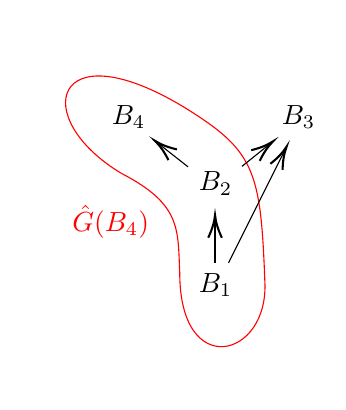
\begin{tikzpicture}[x=0.75pt,y=0.75pt,yscale=-1,xscale=1]
%uncomment if require: \path (0,534); %set diagram left start at 0, and has height of 534

\draw (222,75) node [anchor=north west][inner sep=0.75pt]  [color={rgb, 255:red, 255; green, 0; blue, 0 }  ,opacity=1 ]  {$\hat{G}(B_{4})$};

%Curve Lines [id:da8086917494340398] 
\draw [color={rgb, 255:red, 255; green, 0; blue, 0 }  ,draw opacity=1 ]   (277,29) .. controls (311,50) and (314,59) .. (316,113) ;
%Curve Lines [id:da21472780558540894] 
\draw [color={rgb, 255:red, 255; green, 0; blue, 0 }  ,draw opacity=1 ]   (247,61) .. controls (202,34) and (214,-9) .. (277,29) ;
%Curve Lines [id:da2557925845138229] 
\draw [color={rgb, 255:red, 255; green, 0; blue, 0 }  ,draw opacity=1 ]   (247,61) .. controls (276,76) and (274,88) .. (275,109) ;
%Curve Lines [id:da06777553579467122] 
\draw [color={rgb, 255:red, 255; green, 0; blue, 0 }  ,draw opacity=1 ]   (316,113) .. controls (318,150) and (275,161) .. (275,109) ;


% Text Node
\draw (241,27) node [anchor=north west][inner sep=0.75pt]    {$B_{4}$};
% Text Node
\draw (283,59) node [anchor=north west][inner sep=0.75pt]    {$B_{2}$};
% Text Node
\draw (323,27) node [anchor=north west][inner sep=0.75pt]    {$B_{3}$};
% Text Node
\draw (283,108) node [anchor=north west][inner sep=0.75pt]    {$B_{1}$};
% Connection
\draw    (279,57.79) -- (264.57,46.45) ;
\draw [shift={(263,45.21)}, rotate = 38.16] [color={rgb, 255:red, 0; green, 0; blue, 0 }  ][line width=0.75]    (10.93,-3.29) .. controls (6.95,-1.4) and (3.31,-0.3) .. (0,0) .. controls (3.31,0.3) and (6.95,1.4) .. (10.93,3.29)   ;
% Connection
\draw    (305,57.54) -- (318.44,46.72) ;
\draw [shift={(320,45.46)}, rotate = 141.17] [color={rgb, 255:red, 0; green, 0; blue, 0 }  ][line width=0.75]    (10.93,-3.29) .. controls (6.95,-1.4) and (3.31,-0.3) .. (0,0) .. controls (3.31,0.3) and (6.95,1.4) .. (10.93,3.29)   ;
% Connection
\draw    (292,83) -- (292,104) ;
\draw [shift={(292,81)}, rotate = 90] [color={rgb, 255:red, 0; green, 0; blue, 0 }  ][line width=0.75]    (10.93,-3.29) .. controls (6.95,-1.4) and (3.31,-0.3) .. (0,0) .. controls (3.31,0.3) and (6.95,1.4) .. (10.93,3.29)   ;
% Connection
\draw    (298.5,104) -- (325.61,49.79) ;
\draw [shift={(326.5,48)}, rotate = 116.57] [color={rgb, 255:red, 0; green, 0; blue, 0 }  ][line width=0.75]    (10.93,-3.29) .. controls (6.95,-1.4) and (3.31,-0.3) .. (0,0) .. controls (3.31,0.3) and (6.95,1.4) .. (10.93,3.29)   ;

\end{tikzpicture}

\end{center}

Observe: Given a resampling table $R$, $\hat{G}(B_t)$ explains the values of $\var{B_t}$ before \& after resampling $B_t$.\pause\spadding

\follows we have an injective mapping!
\end{block}
\end{frame}

\begin{frame}{Counting Resamples}
Do we map resamples to \emph{all} witness DAGs?\pause\par
No! \follows we can improve our counting!\pause\spadding

\begin{itemize}
    \item $\hat{G}(B_i)$ always has a single sink (set denoted $\G$)\pause
    \item Given resampling table $R$, do all single-sink witness DAGs $G$ correspond to a possible resample?\pause
    
    \follows No! \pause$G$ \& $R$ must be \b{compatible} (set denoted $\compat{\G}{R}$)\pause\spadding
    
    \underline{Note}: $\Pr[R \sim D]{\text{$G$ \& $R$ compatible}} \pause= \prod_{B \in G} \law(B) \pause\eqdef \w(G)$.
\end{itemize}\pause\spadding

\follows for fixed resampling table $R$, at most $|\compat{\G}{R}|$ resamplings\pause

\vspace{-1.5em}\begin{align*}
    \E{|\compat{\G}{R}|} \pause= \sum_{G \in \G} \Pr{\text{$G$ \& $R$ compatible}} \pause= \sum_{G\in\G} \w(G) \eqdef \underbrace{\w(\G) \pause < \infty}_{\text{\b{Shearer Criterion}}}.
\end{align*}
\end{frame}

\section{A Deterministic Algorithm}
\begin{frame}{Plan}
\tableofcontents[currentsection, sectionstyle=show/shaded, hideothersubsections]
\end{frame}

\subsection{Likely \& Unlikely Resamples}
\begin{frame}{Likely \& Unlikely Resamples}
Want to find resampling table $R$ such that $|\compat{\G}{R}|$ is polynomial.\pause\par
Idea: choose $R$ such that unlikely resamples are avoided!

\begin{columns}[T]
\begin{column}{.55\textwidth}
\g{Example}\quad $\w(G) = \only<2-3>{\nicefrac{1}{4}}\only<4>{\nicefrac{1}{16}}\only<5->{\nicefrac{1}{32}}$.\vspace{0.3em}

\only<6->{For a threshold $\tau \in [0,1]$, \begin{itemize} % TODO: L & U are subsets of collectible witness DAGs
    \item let $\L \subseteq \G$ be the set of \b{likely} witness DAGs, $\w(G) \geq \tau$\only<7->{;
    \item let $\U \subseteq \G$ be the set of \b{(most likely) unlikely} witness DAGs, $\w(G) < \tau$ such that all prefixes are likely.}
\end{itemize}}

\only<8->{\underline{Note}: Fixing resampling table $R$, if $\compat{\U}{R} = \emptyset$, then $\compat{\G}{R} \subseteq \compat{\L}{R}$.}
\end{column}
\begin{column}{.36\textwidth}
\centering


\tikzset{every picture/.style={line width=0.75pt}} %set default line width to 0.75pt        

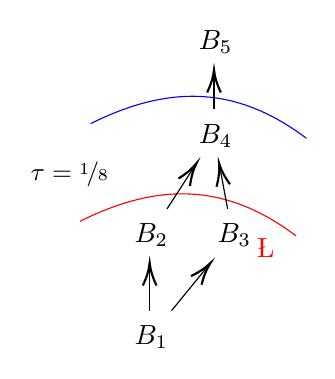
\begin{tikzpicture}[x=0.75pt,y=0.75pt,yscale=-1,xscale=1]
%uncomment if require: \path (0,534); %set diagram left start at 0, and has height of 534

%Curve Lines [id:da3428774655789326] 
\onslide<6->{\draw [color={rgb, 255:red, 255; green, 0; blue, 0 }  ,draw opacity=1 ]   (253,380) .. controls (293,360) and (325,363) .. (357,387) ;}
%Curve Lines [id:da41651271023154823] 
\onslide<7->{\draw [color={rgb, 255:red, 0; green, 0; blue, 255 }  ,draw opacity=1 ]   (258,333) .. controls (298,313) and (330,316) .. (362,340) ;}

% Text Node
\onslide<2,4->{\draw (278,380) node [anchor=north west][inner sep=0.75pt]    {$B_{2}$};}
\onslide<3>{\draw (278,380) node [anchor=north west][inner sep=0.75pt] [opacity=0.2  ]    {$B_{2}$};}
% Text Node
\onslide<4->{\draw (309,332) node [anchor=north west][inner sep=0.75pt]    {$B_{4}$};}
\onslide<2-3>{\draw (309,332) node [anchor=north west][inner sep=0.75pt] [opacity=0.2  ]    {$B_{4}$};}
% Text Node
\draw (278,429) node [anchor=north west][inner sep=0.75pt]    {$B_{1}$};
% Text Node
\onslide<3->{\draw (318,380) node [anchor=north west][inner sep=0.75pt]    {$B_{3}$};}
\onslide<2>{\draw (318,380) node [anchor=north west][inner sep=0.75pt] [opacity=0.2  ]    {$B_{3}$};}
% Text Node
\onslide<5->{\draw (309,287) node [anchor=north west][inner sep=0.75pt]    {$B_{5}$};}
\onslide<2-4>{\draw (309,287) node [anchor=north west][inner sep=0.75pt] [opacity=0.2  ]    {$B_{5}$};}
% Connection 1
\onslide<2,4->{\draw    (286.5,402) -- (286.5,423) ;
\draw [shift={(286.5,400)}, rotate = 90] [color={rgb, 255:red, 0; green, 0; blue, 0 }  ][line width=0.75]    (10.93,-3.29) .. controls (6.95,-1.4) and (3.31,-0.3) .. (0,0) .. controls (3.31,0.3) and (6.95,1.4) .. (10.93,3.29)   ;}
\onslide<3>{\draw [opacity=0.2  ]    (286.5,402) -- (286.5,423) ;
\draw [shift={(286.5,400)}, rotate = 90] [color={rgb, 255:red, 0; green, 0; blue, 0 },opacity=0.2  ][line width=0.75]    (10.93,-3.29) .. controls (6.95,-1.4) and (3.31,-0.3) .. (0,0) .. controls (3.31,0.3) and (6.95,1.4) .. (10.93,3.29)   ;}
% Connection 3
\onslide<4->{\draw    (294.9,374) -- (308.02,353.68) ;
\draw [shift={(309.1,352)}, rotate = 122.86] [color={rgb, 255:red, 0; green, 0; blue, 0 }  ][line width=0.75]    (10.93,-3.29) .. controls (6.95,-1.4) and (3.31,-0.3) .. (0,0) .. controls (3.31,0.3) and (6.95,1.4) .. (10.93,3.29)   ;}
\onslide<2-3>{\draw [opacity=0.2  ]    (294.9,374) -- (308.02,353.68) ;
\draw [shift={(309.1,352)}, rotate = 122.86] [color={rgb, 255:red, 0; green, 0; blue, 0 },opacity=0.2  ][line width=0.75]    (10.93,-3.29) .. controls (6.95,-1.4) and (3.31,-0.3) .. (0,0) .. controls (3.31,0.3) and (6.95,1.4) .. (10.93,3.29)   ;}
% Connection 4
\onslide<4->{\draw    (324.06,374) -- (320.31,353.97) ;
\draw [shift={(319.94,352)}, rotate = 79.38] [color={rgb, 255:red, 0; green, 0; blue, 0 }  ][line width=0.75]    (10.93,-3.29) .. controls (6.95,-1.4) and (3.31,-0.3) .. (0,0) .. controls (3.31,0.3) and (6.95,1.4) .. (10.93,3.29)   ;}
\onslide<2-3>{\draw [opacity=0.2  ]    (324.06,374) -- (320.31,353.97) ;
\draw [shift={(319.94,352)}, rotate = 79.38] [color={rgb, 255:red, 0; green, 0; blue, 0 },opacity=0.2  ][line width=0.75]    (10.93,-3.29) .. controls (6.95,-1.4) and (3.31,-0.3) .. (0,0) .. controls (3.31,0.3) and (6.95,1.4) .. (10.93,3.29)   ;}
% Connection 2
\onslide<3->{\draw    (297.11,423) -- (314.62,401.55) ;
\draw [shift={(315.89,400)}, rotate = 129.23] [color={rgb, 255:red, 0; green, 0; blue, 0 }  ][line width=0.75]    (10.93,-3.29) .. controls (6.95,-1.4) and (3.31,-0.3) .. (0,0) .. controls (3.31,0.3) and (6.95,1.4) .. (10.93,3.29)   ;}
\onslide<2>{\draw [opacity=0.2  ]    (297.11,423) -- (314.62,401.55) ;
\draw [shift={(315.89,400)}, rotate = 129.23] [color={rgb, 255:red, 0; green, 0; blue, 0 },opacity=0.2  ][line width=0.75]    (10.93,-3.29) .. controls (6.95,-1.4) and (3.31,-0.3) .. (0,0) .. controls (3.31,0.3) and (6.95,1.4) .. (10.93,3.29)   ;}
% Connection 5
\onslide<5->{\draw    (317.5,326) -- (317.5,309) ;
\draw [shift={(317.5,307)}, rotate = 90] [color={rgb, 255:red, 0; green, 0; blue, 0 }  ][line width=0.75]    (10.93,-3.29) .. controls (6.95,-1.4) and (3.31,-0.3) .. (0,0) .. controls (3.31,0.3) and (6.95,1.4) .. (10.93,3.29)   ;}
\onslide<2-4>{\draw [opacity=0.2  ]    (317.5,326) -- (317.5,309) ;
\draw [shift={(317.5,307)}, rotate = 90] [color={rgb, 255:red, 0; green, 0; blue, 0 },opacity=0.2  ][line width=0.75]    (10.93,-3.29) .. controls (6.95,-1.4) and (3.31,-0.3) .. (0,0) .. controls (3.31,0.3) and (6.95,1.4) .. (10.93,3.29)   ;}

% \draw (250,287) node [anchor=north west][inner sep=0.75pt]    {$G$};

% Text Node
\onslide<6->{\draw (228,350) node [anchor=north west][inner sep=0.75pt]  [font=\small,color={rgb, 255:red, 0; green, 0; blue, 0 }  ,opacity=1 ]  {$\tau =\nicefrac{1}{8}$};}

% Text Node
\onslide<6->{\draw (337,387) node [anchor=north west][inner sep=0.75pt]  [color={rgb, 255:red, 255; green, 0; blue, 0 }  ,opacity=1 ]  {$\L$};}
% Text Node
\onslide<7->{\draw (335,338) node [anchor=north west][inner sep=0.75pt]  [color={rgb, 255:red, 0; green, 0; blue, 255 }  ,opacity=1 ]  {$\U$};}

\end{tikzpicture}

\flushright\small $G$, suppose $\law \equiv \nicefrac{1}{2}$.
\end{column}
\end{columns}\spadding

\only<9->{\follows need to trade $\tau$!}
\end{frame}

\begin{frame}{Finding Resampling Table avoiding $\U$}
Using the method of conditional expectation, we find $R$ such that \vspace{-0.5em}\begin{align*}
    |\compat{\U}{R}| \leq \E[R \sim D]{|\compat{\U}{R}|} \pause = \w(\U).
\end{align*}\pause

\vspace{-1.8em}\follows if we choose $\tau$ such that $\w(\U) < 1$,\par then $\compat{\U}{R} = \emptyset$ and $\compat{\G}{R} \subseteq \compat{\L}{R}$.\pause\padding

But can $R$ be computed efficiently?\pause\spadding

\underline{Observe}: The MT algorithm uses at most as many columns as the size of the largest witness DAG in $\L$\pause, which is at most $|\L|$.\pause\spadding

For each cell of $R$, choose one of $|\Sigma|$ values to minimize the conditional probability of $G$ \& $R$ being compatible for each $G \in \U$.\pause\spadding

\follows $\O{n |\L| \cdot |\Sigma| \cdot |\L| T \cdot |\U|}$\pause, where $T$ is the runtime of computing conditional probabilities of bad-events given a partial resampling table.\pause\par
Also need to generate $\U$, which can be done in $\poly{|\U|}$ time.
\end{frame}

\begin{frame}{Choosing the Threshold}
Can we choose $\tau$ such that $\w(\U) < 1$ and $\U$ and $\L$ are of polynomial size?\pause

\begin{enumerate}
    \item What is the largest $\tau$ guaranteeing $\w(\U) < 1$?\pause\spadding
    
    For $G \in \U$, we know $\w(G) < \tau$.\pause\par
    \underline{Note}: For $\epsilon > 0$, $\w(G) = \epsw(G)^{\nicefrac{1}{(1-\epsilon)}} \pause< \tau^\epsilon \epsw(G)$\par if we choose $\U$ and $\L$ based on $\epsw$ (this we do from now on!).\pause\par
    \follows $\w(\U) < \tau^\epsilon \epsw(\U)$.\pause\par
    \follows for $\tau \leq \epsw(\U)^{-\nicefrac{1}{\epsilon}} \eqdef \taumax$, we have $\w(\U) < 1$.\pause
    
    \vspace{0.3em}\begin{columns}[T]
    \begin{column}{0.4\textwidth}
    How do we compute $\tau$?\pause\par
    Use exponential backoff!
    
    \g{Example}\quad $\tau = \only<9-10>{2^0 = 1}\only<11>{2^{-1} = \nicefrac{1}{2}}\only<12>{2^{-2} = \nicefrac{1}{4}}\only<13->{2^{-3} = \nicefrac{1}{8}}$.\pause\vspace{0.25em}
    
    \only<14->{\follows $\tau \geq \frac{1}{2} \taumax$}\spadding
    
    \only<15->{Are $\U$ and $\L$ of polynomial size?}
    \end{column}
    \begin{column}{0.12\textwidth}
    \centering


\tikzset{every picture/.style={line width=0.75pt}} %set default line width to 0.75pt        

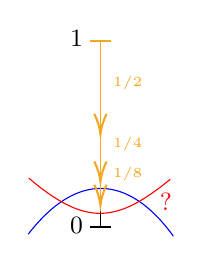
\begin{tikzpicture}[x=0.75pt,y=0.75pt,yscale=-1,xscale=1,rotate=180,scale=0.9]
%uncomment if require: \path (0,534); %set diagram left start at 0, and has height of 534

%Straight Lines [id:da8648942484395017] 
\draw    (590.4,100.4) -- (590.4,200.07) ;
\draw [shift={(590.4,200.07)}, rotate = 270] [color={rgb, 255:red, 245; green, 166; blue, 35 }  ][line width=0.75]    (0,5.59) -- (0,-5.59)   ;
\draw [shift={(590.4,100.4)}, rotate = 270] [color={rgb, 255:red, 0; green, 0; blue, 0 }  ][line width=0.75]    (0,5.59) -- (0,-5.59)   ;

% Text Node
\draw (608,107) node [anchor=north west][inner sep=0.75pt]  [font=\small]  {$0$};
% Text Node
\draw (608,207) node [anchor=north west][inner sep=0.75pt]  [font=\small]  {$1$};
% Text Node
\onslide<8->{\draw (584,102) node [anchor=north west][inner sep=0.75pt]  [font=\small,color={rgb, 255:red, 0; green, 0; blue, 255 }  ,opacity=1 ]  {$\taumax$};}
% Text Node
\onslide<9->{\draw (585,183) node [anchor=north west][inner sep=0.75pt]  [font=\footnotesize,color={rgb, 255:red, 245; green, 166; blue, 35 }  ,opacity=1 ]  {$1/2$};}
% Text Node
\onslide<10->{\draw (585,150) node [anchor=north west][inner sep=0.75pt]  [font=\footnotesize,color={rgb, 255:red, 245; green, 166; blue, 35 }  ,opacity=1 ]  {$1/4$};}
% Text Node
\onslide<11->{\draw (585,134) node [anchor=north west][inner sep=0.75pt]  [font=\footnotesize,color={rgb, 255:red, 245; green, 166; blue, 35 }  ,opacity=1 ]  {$1/8$};}
% Text Node
\onslide<12->{\draw (560,120) node [anchor=north west][inner sep=0.75pt]  [font=\small,color={rgb, 255:red, 255; green, 0; blue, 0 }  ,opacity=1 ] [align=left] {?};}

%Curve Lines [id:da5356270327996431] 
\onslide<8->{\draw [color={rgb, 255:red, 0; green, 0; blue, 255 }  ,draw opacity=1 ]   (551.4,95.73) .. controls (575.4,128.73) and (603.07,130.4) .. (629.07,96.73) ;}

%Straight Lines [id:da42007517029648045] 
\onslide<9->{\draw [color={rgb, 255:red, 245; green, 166; blue, 35 }  ,draw opacity=1 ]   (590.4,200.07) -- (590.4,152.23) ;
\draw [shift={(590.4,150.23)}, rotate = 90] [color={rgb, 255:red, 245; green, 166; blue, 35 }  ,draw opacity=1 ][line width=0.75]    (10.93,-3.29) .. controls (6.95,-1.4) and (3.31,-0.3) .. (0,0) .. controls (3.31,0.3) and (6.95,1.4) .. (10.93,3.29)   ;}
%Straight Lines [id:da4473125650369483] 
\onslide<10->{\draw [color={rgb, 255:red, 245; green, 166; blue, 35 }  ,draw opacity=1 ]   (590.4,150.23) -- (590.4,126.73) ;
\draw [shift={(590.4,124.73)}, rotate = 90] [color={rgb, 255:red, 245; green, 166; blue, 35 }  ,draw opacity=1 ][line width=0.75]    (10.93,-3.29) .. controls (6.95,-1.4) and (3.31,-0.3) .. (0,0) .. controls (3.31,0.3) and (6.95,1.4) .. (10.93,3.29)   ;}
%Straight Lines [id:da921748453412278] 
\onslide<11->{\draw [color={rgb, 255:red, 245; green, 166; blue, 35 }  ,draw opacity=1 ]   (590.4,124.73) -- (590.4,114.23) ;
\draw [shift={(590.4,112.23)}, rotate = 90] [color={rgb, 255:red, 245; green, 166; blue, 35 }  ,draw opacity=1 ][line width=0.75]    (10.93,-3.29) .. controls (6.95,-1.4) and (3.31,-0.3) .. (0,0) .. controls (3.31,0.3) and (6.95,1.4) .. (10.93,3.29)   ;}

%Curve Lines [id:da40449977786973723] 
\onslide<12->{\draw [color={rgb, 255:red, 255; green, 0; blue, 0 }  ,draw opacity=1 ]   (553.07,126.07) .. controls (581.4,103.07) and (597.73,100.4) .. (628.73,126.73) ;}


\end{tikzpicture}

    \end{column}
    \begin{column}{0\textwidth}
    \end{column}
    \end{columns}
\end{enumerate}
\end{frame}

\begin{frame}{Choosing the Threshold}
    \begin{enumerate}
        \setcounter{enumi}{1}
        \item Is $\U \cup \L$ of polynomial size?\pause\spadding
        
        \underline{Observe}: Removing the sink $B$ from $G \in \U \cup \L$,\par we have $\epsw(G - B) \geq \tau$.\pause\spadding
        
        This allows us to count the elements! \vspace{-0.5em}\begin{align*}
        %     \sum_{\substack{G \in \U \cup \L \\ \text{with sink $B$}}} 1 \leq \sum_{\substack{G \in \U \cup \L \\ \text{with sink $B$}}} \frac{\epsw(G - B)}{\tau} \leq \sum_{\substack{G \in \U \cup \L \\ \text{with sink $B$}}} \frac{\epsw(G)}{\tau}
        % \end{align*} Summing over all $B \in \B$, \vspace{-0.5em}\begin{align*}
            |\U \cup \L| &\leq \frac{\epsw(\U \cup \L)}{\tau} \pause\leq \frac{\epsw(\G)}{\tau} \\
                         &\pause\leq \frac{2 \epsw(\G)}{\taumax} = 2 \epsw(\G)^{1+\frac{1}{\epsilon}}.
        \end{align*}
    \end{enumerate}
\end{frame}

\subsection{The Algorithm}
\begin{frame}{The Algorithm}
\begin{algorithm}[H]
\TitleOfAlgo{Deterministic MT-Algorithm}
Select threshold $\tau$ such that $\w(\U) < 1$ and $|\U \cup \L| \leq 2 \epsw(\G)^{1+\frac{1}{\epsilon}}$\;\pause
Generate the witness DAGs $\U$\;\pause
Find resampling table $R$ avoiding $\U$\;\pause
Run the deterministic MT algorithm on $R$\;
\end{algorithm}\pause\spadding

We have seen that the final step takes at most $|\compat{\G}{R}| \leq |\compat{\L}{R}|$ iterations!
\end{frame}

% \subsection{Counting Resamples with Witness DAGs}
% \subsubsection{What are Witness DAGs?}
% \begin{frame}{Frame Title}
    
% \end{frame}
% \subsubsection{From Witness DAGs to the Resampling Table to the MT Algorithm}
% \begin{frame}{Frame Title}
    
% \end{frame}
% \subsection{Shearer's Criterion}
% \begin{frame}{Frame Title}
    
% \end{frame}

% \section{A Deterministic Algorithm}
% \begin{frame}{Plan}
% \tableofcontents[currentsection, sectionstyle=show/shaded, hideothersubsections]
% \end{frame}
% \subsection{Shearer's Criterion with Slack}
% \begin{frame}{Frame Title}
    
% \end{frame}
% \subsection{Counting Witness DAGs}
% \begin{frame}{Frame Title}
    
% \end{frame}
% \subsection{Analyzing the Deterministic Algorithm}
% \begin{frame}{Frame Title}
    
% \end{frame}
% \subsection{Pre-processing the Witness DAG and Crisper Results}
% \begin{frame}{Frame Title}
    
% \end{frame}

% \section{Outlook: A Parallel Algorithm and the MT-distribution}
% \begin{frame}{Plan}
% \tableofcontents[currentsection, sectionstyle=show/shaded, hideothersubsections]
% \end{frame}
% \begin{frame}{Frame Title}
    
% \end{frame}

\begin{frame}{}
    \centering \large
    Thanks for your attention!
    Questions?
\end{frame}

\end{document}